\section{\label{sec:mass_in_sm}Neutrinos, Standard Model and Mass Terms}

Although the SM has been marvelously successful for the last couple of decades, in 1998 the breakthrough regarding the neutrino flavour oscillations threw a spanner in the works. The subject of neutrino mass underlies many of the current leading questions in particle physics. Why is there more matter than anti-matter? There are some indications that understanding the mechanism of neutrino mass could help solve this. Why are the neutrinos so light? Figure~\ref{fig:sm_fremion_mass} is a plot of the neutrino mass compared to the mass of the other charged leptons. The neutrino mass is roughly a factor of a million less than the other particles, which only differ in mass by at most a thousand.


\begin{figure}[!ht]
    \centering
    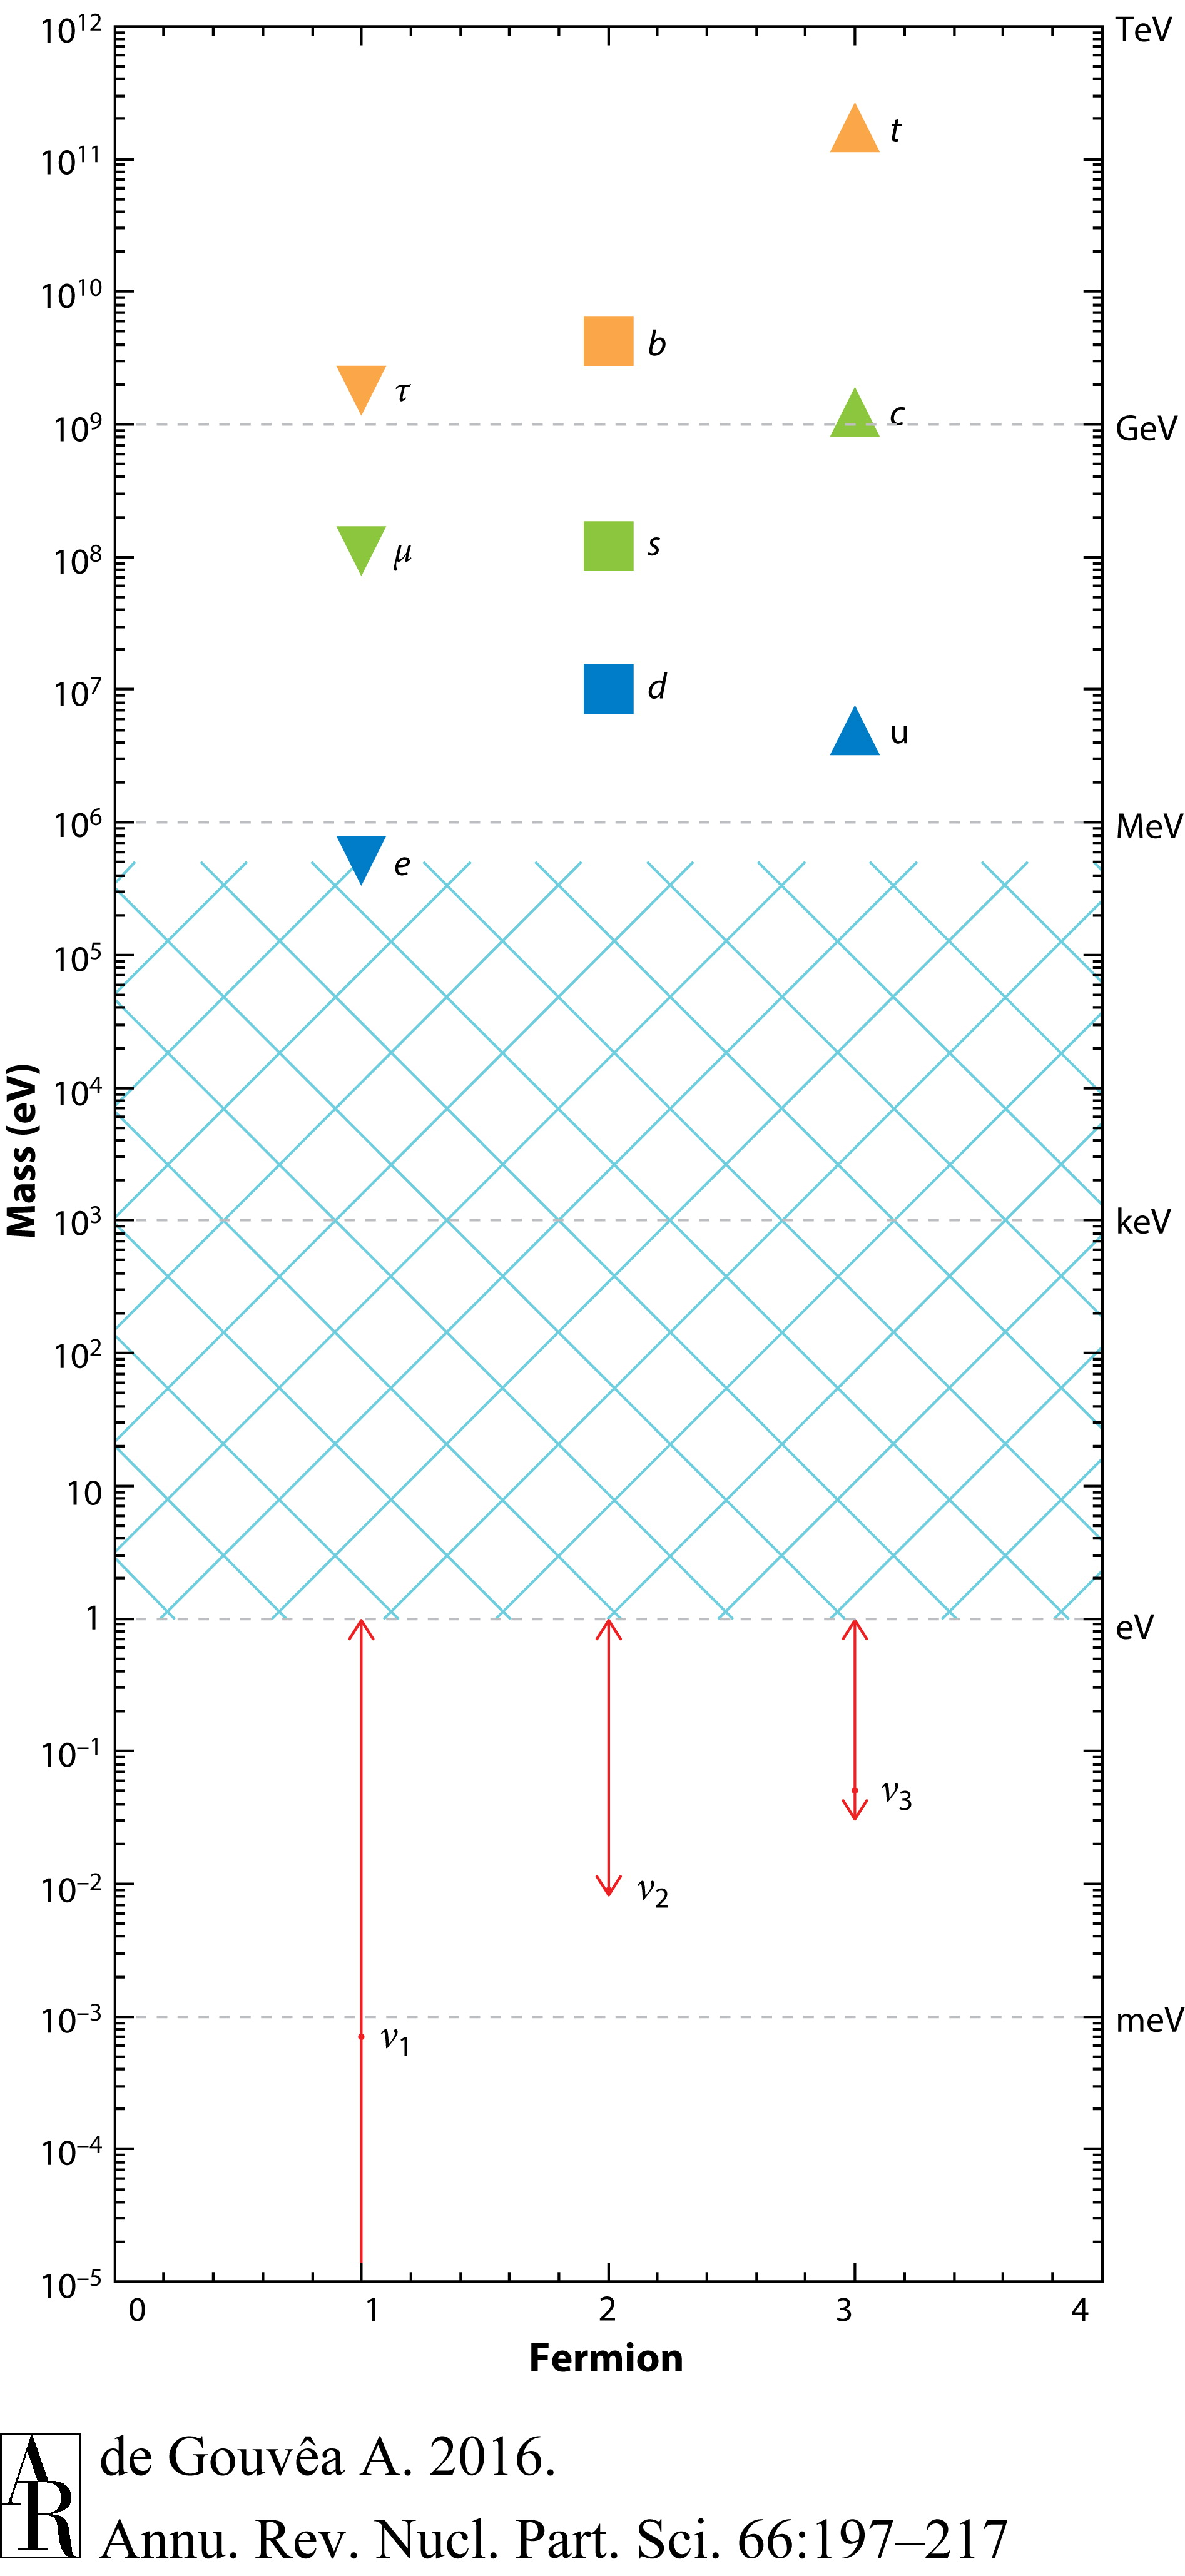
\includegraphics[height=0.7\textwidth]{sm_mass.jpeg}
    \caption{The Standard Model fermion masses.The arrows indicate the allowed ranges for the neutrino masses, assuming a so-called normal mass ordering: $m_{23} ^2> m_{22}^2 > m_{21}^2$ (Ref~\onlinecite{Gouvêa_2016})}
    \label{fig:sm_fremion_mass}
\end{figure}
We will discuss briefly how some of these questions may be solved.  



\subsection{Dirac Mass}
The standard way to include mass in Standard Model is through Dirac Mass Terms in the Lagrangian:
\begin{equation}
        m\overline {\psi} \psi
\end{equation}
If we decompose the dirac spinor \(\psi\) into it's left and right handed-chiral states, we may rewrite the mass term above as
\begin{equation}
    \begin{aligned}
        m\overline {\psi} \psi = m\overline{(\psi_L + \psi _R)}(\psi_L + \psi _R)\\
         = m\overline {\psi} _L \psi_R + m\overline {\psi}_R \psi_L
    \end{aligned}
\end{equation}
above we used the property \(\overline {\psi}_L \psi_L =\overline {\psi}_R \psi_R = 0\).

The important point to note is that a non-zero Dirac mass requires a particle to have both a left-and right-handed chiral state : in fact the \textsc{Dirac mass can be viewed as being the coupling constant
between the two chiral components}. Also, observe this formalism is not gauge invariant.

To begin with, remember that the left-handed neutrino field \(\nu _L\) in the Standard Model is a part of a doublet of a left-handed weak field, other being the left-handed electron: \(\begin{pmatrix}e \\ \nu\end{pmatrix}_L\). These fields are distinguised from each other only by their \emph{weak charge}, also called \emph{weak isospin} \(T_3\). The right-handed particle fields are singlet fields, with no weak charge at all (and hence right-handed particle fields can’t couple to the $W$ bosons, in much the same way as neutrinos can’t couple to photons as they are electrically
neutral

The field \(e_L\) has a weak charge of $T_3 = - \frac{1}{2}$ and an electric charge $Q = -1$. Now, a consequence of being gauge invariant is that all terms in the Lagrangian are neutrally charged; both electrically and from the point of view of the weak interaction. Now consider the Dirac mass term for an electron: $m_e e_R e_L$ . The charges on each of the charged lepton fields and the overall term are shown in Table~\ref{tab:charges_sm}.
Note that ``\textit{adjointing}"  a field flips the sign of the charge.
\begin{table}[!h]
    \centering
    \begin{tabular}{|c|c|c|c|c|}\hline
    & $e_L$ & $e_R$ & $\overline {e}_R$ & $\overline {e}_R\overline {e}_L$\\\hline
    $Q$ & $-1$ & $-1$ & $+1$ & $0$\\
    $T_3$ & $-1/2$ & $0$ & $0$ & $-1/2$  \\\hline
    \end{tabular}
    \caption{Charges of fields in the electron Dirac mass term}
    \label{tab:charges_sm}
\end{table}
Since the dirac mass terms are not gauge invariant, we need to add a field to mass term which (i) has \(Q = 0\) (ii) has \(T_3 = 1/2\). This field would be electrically neutral but part of weak doublet, just like the left-handed electron field. This field will turn out to be the neutral Higgs boson. With this addition, the Dirac mass term becomes neutrally charged and the term is gauge invariant.

Since we know the neutrino is chirally left-handed, there is good reason to suppose that the neutrino must be massless, as there does not seem to be a right-handed state for the mass term to couple to. However, we now know that the neutrino does have a small mass, so either there must be a right-handed neutrino which only shows up in the standard model to give the neutrino mass, but otherwise cannot be observed as the weak interaction doesn’t couple to it, or there is some other sort  of mass term out there.

By definition Dirac particles come in four distinct types: left- and right-handed particles, and left- and right-handed antiparticles, and are therefore represented by a 4-component Dirac spinor. As we will see in the next section, charged fermions can only have a Dirac type mass. For neutral fermions, however, this need not be the case. Such particles could acquire mass through the \emph{Majorana mass mechanism}.